\documentclass[12pt, a4paper]{article}
\usepackage[francais]{babel}
\usepackage{pgfplots}
\usepackage{caption}
\usepackage{graphicx}
\usepackage[T1]{fontenc}
\usepackage{listings}
\usepackage{geometry}
\usepackage{minted}
\usepackage{array,multirow,makecell}
\usepackage[colorlinks=true,linkcolor=black,anchorcolor=black,citecolor=black,filecolor=black,menucolor=black,runcolor=black,urlcolor=black]{hyperref}
\setcellgapes{1pt}
\makegapedcells
\usepackage{fancyhdr}
\pagestyle{fancy}
\lhead{}
\rhead{}
\chead{}
\rfoot{\thepage}
\lfoot{}
\cfoot{}

\renewcommand{\headrulewidth}{0.4pt}
\renewcommand{\listingscaption}{Code}
\renewcommand{\listoflistingscaption}{Table des codes}
% \usepackage{mathpazo} --> Police à utiliser lors de rapports plus sérieux

\begin{document}
\begin{titlepage}
	\newcommand{\HRule}{\rule{\linewidth}{0.5mm}} 
	\center 
	\textsc{\LARGE iut de colmar}\\[6.5cm] 
	\textsc{\Large SAE3 - ROM}\\[0.5cm] 
	\textsc{\large Année 2022-23}\\[0.5cm]
	\HRule\\[0.75cm]
	{\huge\bfseries Déployer un service de téléphonie}\\[0.4cm]
	\HRule\\[1.5cm]
	\textsc{\large martin baumgaertner}\\[6.5cm] 

	\vfill\vfill\vfill
	{\large\today} 
	\vfill
\end{titlepage}
\newpage
\tableofcontents
\newpage
\section*{Contexte}
L'objectif de CETTE SAE et de créer un service de téléphonies "multi-sites". Je
m'explique. Nous avons à disposition, un serveur Asterisk qui est un serveur de
téléphonie IP. Ce serveur est installé sur une machine virtuelle Debian11. Nous
avons aussi à disposition, 2 téléphones IP matériel qui sont des téléphones SIP. Ces
téléphones sont connectés dans le même réseau que notre serveur IPBX bien entendu. 
Puis, nous avons un troisième téléphone IP mais cette fois-ci sous forme de softphone
qui est un téléphone SIP qui est installé sur un ordinateur. Nous utiliserons 
Linphone. Ce dernier est un logiciel libre et gratuit. Il est disponible sur
Windows, Linux et Mac. Ce softphone est connecté sur le même réseau que notre serveur
IPBX.\\

Chaque membre de la SAE doit choisir un contexte de travail différent. J'ai pour
ma part choisi d'être la table 1, le médecin généraliste. De plus, nous 
avons donc ces 3 postes IP pour illustrer un vrai cabinet. C'est-à-dire que nous
avons un poste physique pour le praticien, un poste physique pour l'assistant et
le softphone pour le secretariat.\\

\section{Objectif 1}
\subsection{Configuration Serveur IPBX}
	\subsubsection{Créer une machine virtuelle Debian11}
	Pour cette SAE, j'ai décidé de choisir d'utiliser WMWare Workstation car c'était
	le logiciel que nous utilisions en cours surtout pendant les TP réseaux en première
	année. J'ai donc crée une VM Debian11. 

	\subsubsection{Installez l'IPBX asterisk via le système de paquets Debian}
	Pour pouvoir installer asterisk, il faut d'abord installer le paquet suivant :\\
	
	\texttt{sudo apt install asterisk}\\

	Une fois Asterisk installé, pour l'utiliser il faut arrêter le service pour pouvoir
	démarrer Asterisk car sinon il y a un conflit. Pour arrêter le service, il faut
	écrire la commande suivante : \texttt{service asterisk stop}. Ensuite, nous
	pouvons démarrer Asterisk avec la commande suivante : \texttt{asterisk -vvvvc}.


	\subsubsection{Pour le service IPBX, déclarez les différents postes SIP}
	Pour déclarer les différents postes SIP, j'ai donc écris les commandes suivantes
	dans les fichiers de configuration de Asterisk.\\

	Premièrement, \textbf{pjsip.conf} :
	\begin{figure}[h]
		\centering
		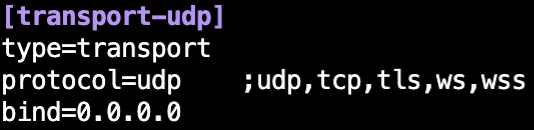
\includegraphics[width=0.8\textwidth]{img/pjsip.png}
		\caption{Configuration de pjsip.conf}
		\label{fig:pjsip}
	\end{figure}

	\newpage
	Puis, \textbf{pjsip wizard.conf} :
	\begin{figure}[h]
		\centering
		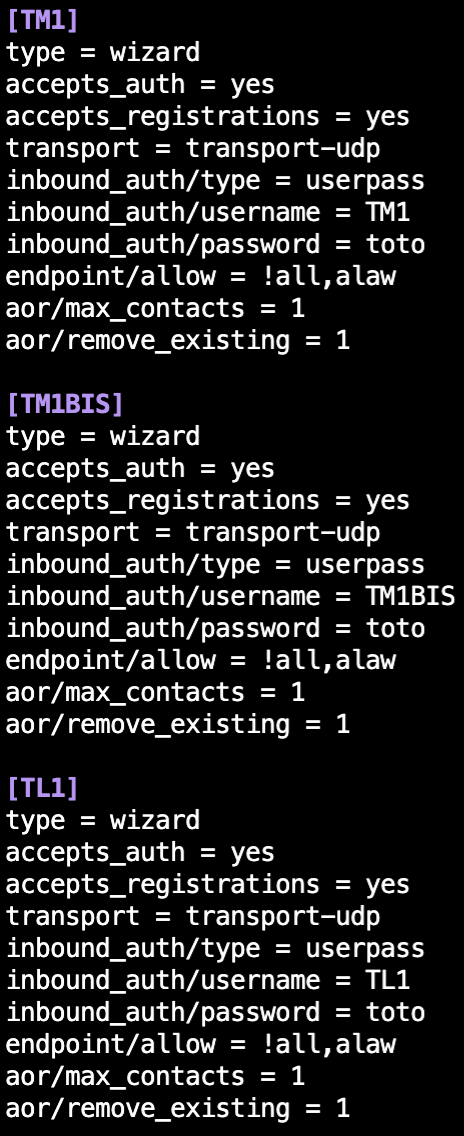
\includegraphics[width=0.4\textwidth]{img/wizard.png}
		\caption{Configuration de pjsip wizard.conf}
		\label{fig:wiz}
	\end{figure}

	Nous avons ici donc la configuration de tous les téléphones. A chaque fois, j'ai
	donc déclaré un téléphone avec son numéro de téléphone, son mot de passe et son
	nom d'utilisateur. Certaines lignes permettent de faire différentes choses
	essentielles au bon fonctionnement du serveur Asterisk. Comme par exmeple, 
	\texttt{aor/remove existing = 1} qui permet de
	supprimer les anciennes configurations qui auraient pu être associés au même nom.\\

	\subsubsection{Pour le service IPBX, créer le plan de numérotation}
	J'ai donc crée le plan de numérotation de la même manière que nous l'avons vu en cours
	et en TP comme peut en témoigner la capture d'écran suivante en rajoutant bien 
	entendu ces lignes dans le contexte \texttt{[default]} :
	\begin{figure}[h]
		\centering
		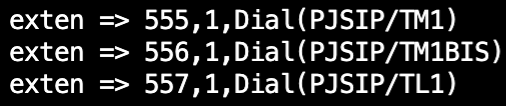
\includegraphics[width=0.7\textwidth]{img/extensions.png}
		\caption{Configuration de extensions.conf}
		\label{fig:ext}
	\end{figure}

\subsection{Configuration Téléphone Clients}
	\subsubsection{Téléphone logiciel Linphone}
	Tout d'abord j'ai voulu configurer linphone sur la machine windows de l'IUT
	sur laquelle j'ai fait ma VM Debian. Cependant, j'ai eu de nombreux problèmes
	Linphone ne fonctionnait pas, même après avoir essayé plusieurs versions. 
	J'ai donc essayé d'utiliser mon ordinateur personnel pour faire cette 
	manipulation. J'ai donc installé Linphone sur mon ordinateur personnel et 
	ça a fonctionné. Pour faire marcher Linphone j'ai utilisé la configuration suivante : \textit{Où 10.129.10.164 est l'IP de mon serveur Asterisk}
	\begin{figure}[h]
		\centering
		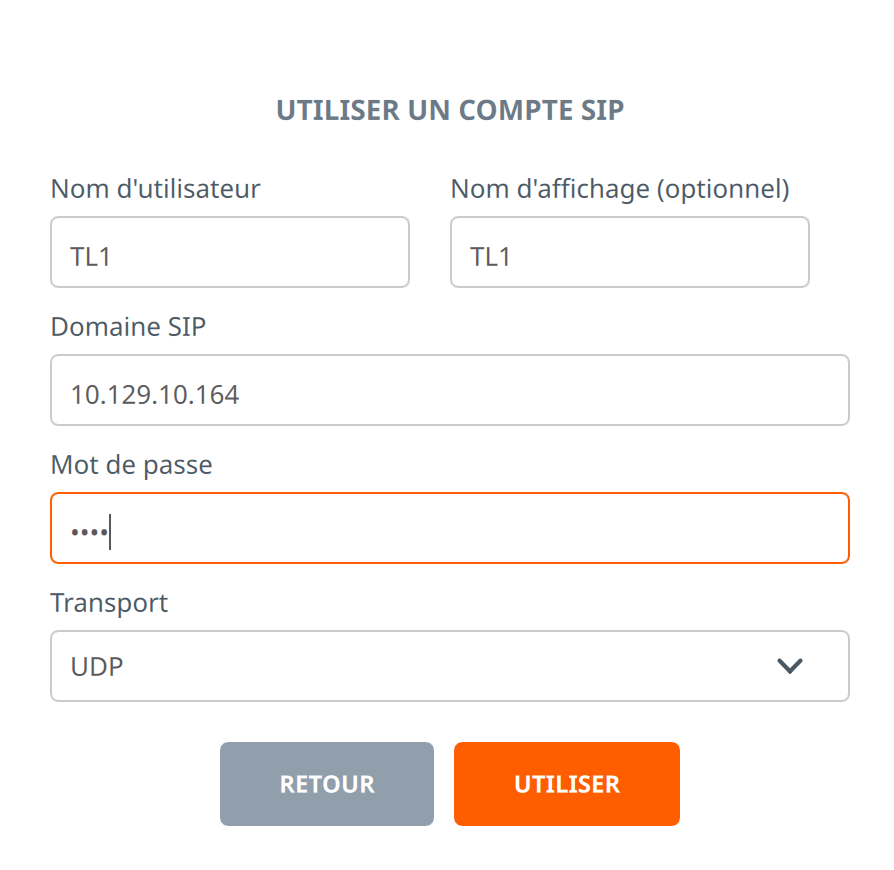
\includegraphics[width=0.5\textwidth]{img/linphone.png}
		\caption{Configuration de Linphone}
		\label{fig:lin}
	\end{figure}

\end{document}